%!TEX root = main.tex

\section{Introduction}
We will be discussing the deflection of light in space from the point of view of general relativiy, and will thus require a way to go from the spacetime $\man$ to a three dimensoinal space.
This is the subject of \textbf{optical geometry}.
We will begin by discussing the generalisation of Fermats principle to spacetime. In order to do concrete (optical geometric) calculations, we will specialize to \textbf{static spacetimes}, which turn out to have Riemannian structure.
In this framework, we will see that gravitational lensing is a global effect, where the topology will determine whether we can have multiple images, what the deflection angles are, etc... This will utilize the so called Gauss Bonnet theorem.

\section{Fermats principle in classical optics}
The first idea (proposed by Herod 10-75CE) is that light takes the shortest path between two points.
Indeed this is the case, however, only for homogeneous media.
More generally, light always takes the shortest path in time.
Let $\gamma: (0,1) \to \reals^3$.
Then the action $S[\gamma] \defn \int_{\gamma} \, dt = \frac{1}{c}\int_{\gamma} n(r) \, dl$ is minimized with respect to the curve $\gamma$, where $n$ is a spatially varying refractive index.
\begin{remark}[]\label{}
Light travels along null geodesics in spacetime, and thus the length is $0$! This means that we have to come up with a new way to formulate Fermats principle in spacetime.
\end{remark}

\begin{definition}[]\label{}
Let $\gamma: I \to \man$ be a curve. Then $\gamma$ is a \textbf{null curve} if $g(\dot{\gamma}(\lambda), \dot{\gamma}(\lambda))=0$ for every $\lambda \in I$.
\end{definition}
%
\begin{definition}[]\label{}
Let $\gamma: I \to \man$ be a curve. Then $\gamma$ is a \textbf{null geodesic} if it is a null curve, and $\nabla_{\dot{\gamma}} \dot{\gamma}$
\end{definition}

\begin{definition}[]\label{}
Let $\gamma: I \to \man$ be a curve. Then the \textbf{$i$'th coordinate image of $\gamma$ under $x$} is a map $\gamma^i_{(x)}: \reals \to \reals$ defined by
\begin{equation}\label{}
\gamma^i_{(x)}(\lambda) \defn (x \circ \gamma)^i (\lambda) = (x_i \circ \gamma) (\lambda)
\end{equation}
\end{definition}
%
\begin{definition}[]\label{}
Let $\gamma: I \to \man$ be a curve. Then the \textbf{velocity field along $\gamma$} is the map $\vg: \reals \to \tanb$ such that $\lambda \mapsto \vg_{(x)}^i (\lambda) \ddx{i} \rvert_{\gamma(\lambda)}$
\end{definition}
%
\begin{proposition}[]\label{}
Let $\gamma: I \to \man$ be a curve, and $\vg$ be the velocity field along $\gamma$. Then
\begin{equation}\label{}
g(\vg(\lambda), \vg(\lambda)) = \vg_{(x)}^{\mu}(\lambda) \vg_{(x)}^{\nu}(\lambda) g_{\mu \nu} \rvert_{\gamma(\lambda)}
\end{equation}
\end{proposition}
%
\begin{theorem}[Fermat \cite{1992grle.book.....S}]\label{}
Let $(\man, g)$ be a spacetime, $S \in \man$ be a source, and $l$ be an observer. Then a smooth null curve $\gamma: (0,1) \to \man$ such that $\gamma(0) = S$ and $\gamma(1) = l(\tau)$ is a null geodesic iff its arrival time $\tau$ is stationary under first order variations of $\gamma$ within the set of smooth null curves from $S$ to $l$.
\end{theorem}
\begin{proof}
$(\implies)$. Consider a family of variances $\eta(\lambda, \epsilon)$ such that $\eta(\cdot, \epsilon) : (0,1) \to \man$, $\eta(0, \epsilon) = S$ for every $\eps \le \abs{\eps_0} \ll 1$, and $\eta(1, \epsilon) = l(\tau_0 + t(\epsilon))$ where $t: \reals \to \reals$ with $t(0)=0$.
Furthermore, let $g(\veta(\lambda, \eps), \veta(\lambda, \eps)) = 0$ for every $\lambda \in (0,1)$, where $\veta$ denotes the velocity field along $\eta(\cdot, \eps)$. We have constructed a family of null variations with fixed beginning and open end.
%
\begin{figure}[!htb]
	\centering
	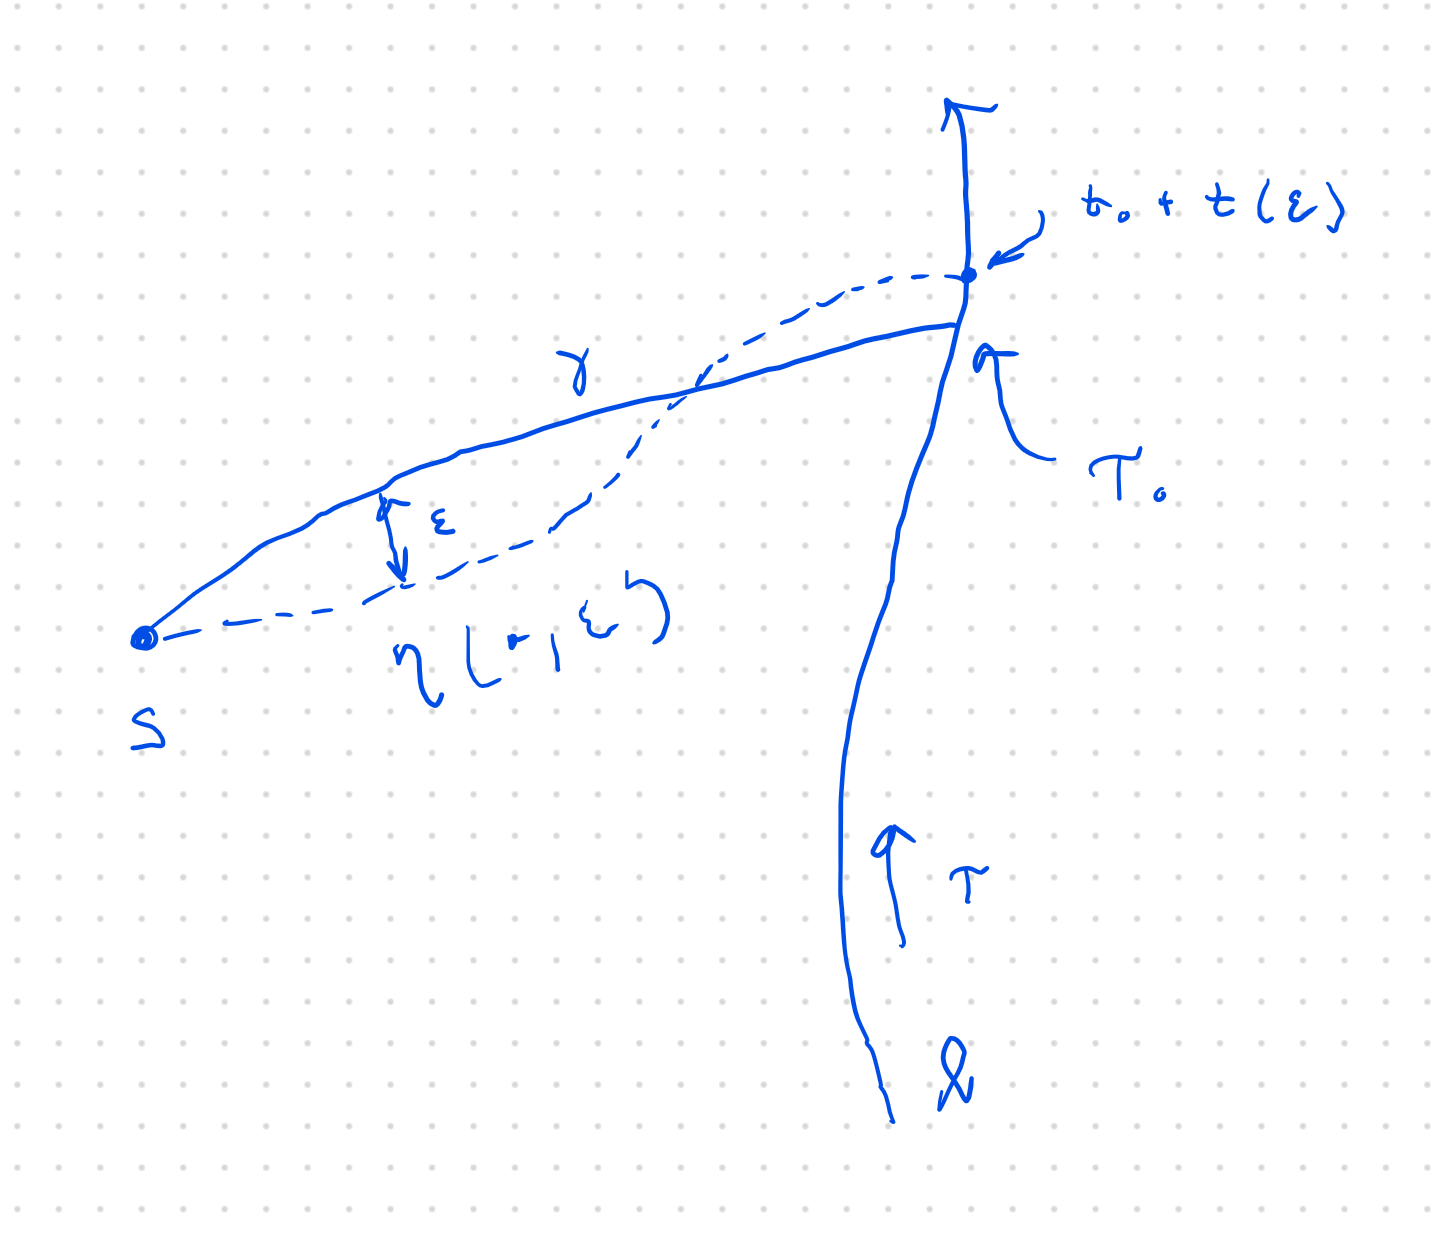
\includegraphics[width=0.5\textwidth]{img/null-variations.png}
	\caption{Family of null variations}
	\label{}
\end{figure}

The action takes the form
\begin{equation}\label{}
S[\gamma_{\eps}] = \int_0^1 L(\eta(\lambda, \eps), \nabla_{\lam} \eta(\lam, \eps)) \, d\lam
\end{equation}
with the Lagrangian
\begin{align*}
L(\eta(\lam, \eps), \veta(\lam, \eps)) &= \frac{1}{2} g (\nabla_{\lam} \eta(\lam, \eps), \nabla_{\lam} \eta(\lam, \eps)) \\
&= \frac{1}{2} g_{\mu, \nu} \rvert_{\gamma(\lam)} \veta^{\mu} (\lam, \eps) \veta^{\nu}(\lam, \eps)
\end{align*}




\end{proof}
